\documentclass[11pt]{article}
\usepackage[margin=1in]{geometry}
\usepackage{amsmath,amssymb}
\usepackage{booktabs}
\usepackage{tabularx}
\usepackage{graphicx}
\usepackage{tikz}
\usetikzlibrary{arrows.meta,positioning,fit,backgrounds}
\graphicspath{{../results/figures/}}

\renewcommand{\thefigure}{S\arabic{figure}}
\renewcommand{\thetable}{S\arabic{table}}

\begin{document}

\begin{center}
{\Large\bfseries Supplementary Information}\\[1ex]
{\large A decentralized neutrosophic decision layer for global-state freshness in microservices architectures}\\[1ex]
Haitham A. El-Ghareeb
\end{center}

\bigskip

\section*{Supplementary Figures}

\setcounter{figure}{0}

\begin{figure}[t]\centering
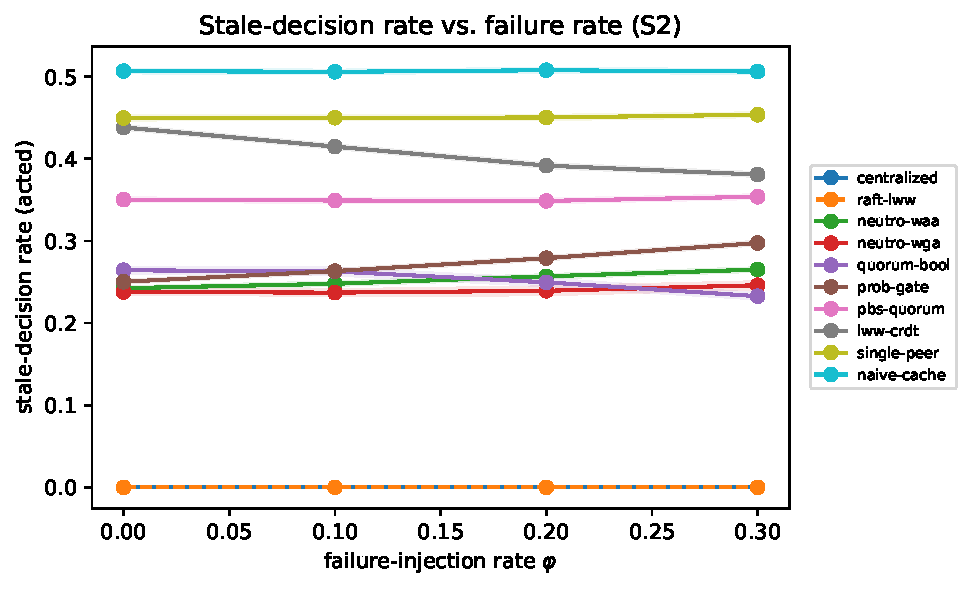
\includegraphics[width=0.7\linewidth]{f2_stale_vs_phi.pdf}
\caption{Stale-decision rate vs.\ failure-injection rate (S2). Bands are 5000-resample bootstrap
95\% CIs.}\label{fig:stale}\end{figure}

\begin{figure}[t]\centering

\includegraphics[width=0.65\linewidth]{f8_signal_richness.pdf}
\caption{RQ1: the indeterminacy axis is well populated and the $(T,I,F)$ decision diverges from a
boolean quorum on a substantial fraction of decisions.}\label{fig:signal}\end{figure}

\begin{figure}[t]\centering

\includegraphics[width=0.8\linewidth]{f5_latency_measured.pdf}
\caption{Measured median decision latency on the real localhost HTTP testbed: local read, single
round-trip, and $R$-peer fan-out tiers. Log scale: naive-cache is a local read ($\approx0.02$\,ms),
dwarfed by the network tiers but fully measured ($n=200$ per cell).}\label{fig:latency}\end{figure}

\begin{figure}[t]\centering

\includegraphics[width=0.8\linewidth]{f10_throughput.pdf}
\caption{Measured throughput (decisions/sec) under concurrent closed-loop load on the real HTTP
testbed.}\label{fig:throughput}\end{figure}

\begin{figure}[t]\centering

\includegraphics[width=0.7\linewidth]{f9_s3_convergence.pdf}
\caption{S3: a fresh clone recovers state by replaying the log; SVNNWGA acceptance trails until
catch-up while SVNNWAA stays available throughout. State-recovery and SVNNWGA acceptance coincide
(dashed line over the thick one).}\label{fig:s3}\end{figure}

\begin{figure}[t]\centering

\includegraphics[width=0.95\linewidth]{f6_sensitivity.pdf}
\caption{Sensitivity of the stale-decision rate to replica count $R$ and cache ratio $\rho$
(S2, $\varphi=0.1$).}\label{fig:sensitivity}\end{figure}

\begin{figure}[t]\centering

\includegraphics[width=0.85\linewidth]{f14_wan_latency.pdf}
\caption{Decision latency on a single-host Docker deployment under \emph{emulated} WAN (Toxiproxy
per-link latency, jitter, and loss): p50 (bar) and p99 (cap), log scale. The wait patterns
(single-hop, majority, $R$-peer fan-out) separate cleanly and the gap grows with link latency; under
$2\%$ loss the tails inflate to the $1$\,s decision deadline, most for the fan-out (it waits for the
slowest of $R$ peers). Real HTTP over proxied sockets; not geo-distributed.}\label{fig:wan}\end{figure}

\begin{figure}[t]\centering

\includegraphics[width=0.95\linewidth]{f15_tuning.pdf}
\caption{Axis B: equal-budget metaheuristic tuning of $[\tau,\text{weights}]$ (seven optimizers, $120$
evaluations each), tuned utility per optimizer (points) versus the uniform-weights baseline (dashed). At
equal budget the optimizers converge---identically on the symmetric S1/S3, within ${\approx}2\%$ on the
asymmetric S2---and tuning beats uniform weights only on S2 ($+10.1\%$); on S1/S3 uniform is already
optimal. No-Free-Lunch: the gain is not an artefact of the optimizer.}\label{fig:tuning}\end{figure}

\begin{figure}[t]
\centering
\resizebox{\ifdim\width>\linewidth\linewidth\else\width\fi}{!}{%
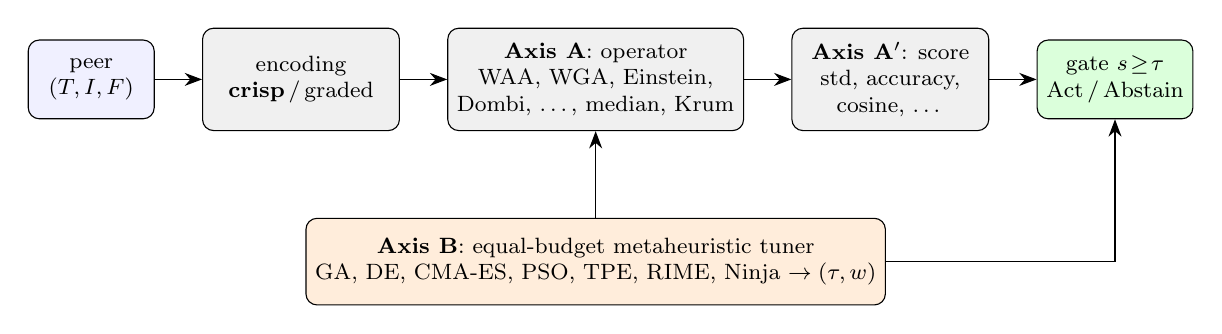
\begin{tikzpicture}[>={Stealth[length=2.2mm]}, font=\footnotesize,
  st/.style={draw,rounded corners,fill=blue!6,align=center,minimum height=10mm,minimum width=16mm},
  ax/.style={draw,rounded corners,fill=gray!12,align=center,minimum height=13mm,minimum width=25mm},
  tn/.style={draw,rounded corners,fill=orange!14,align=center,minimum height=11mm,minimum width=52mm},
  gatebox/.style={draw,rounded corners,fill=green!14,align=center,minimum height=10mm,minimum width=17mm}]
  \node[st] (views) {peer\\$(T,I,F)$};
  \node[ax,right=6mm of views] (enc) {encoding\\\textbf{crisp}\,/\,graded};
  \node[ax,right=6mm of enc] (opA) {\textbf{Axis A}: operator\\WAA, WGA, Einstein,\\Dombi, \dots, median, Krum};
  \node[ax,right=6mm of opA] (scA) {\textbf{Axis A$'$}: score\\std, accuracy,\\cosine, \dots};
  \node[gatebox,right=6mm of scA] (gate) {gate $s\!\ge\!\tau$\\Act\,/\,Abstain};
  \draw[->] (views)--(enc); \draw[->] (enc)--(opA); \draw[->] (opA)--(scA); \draw[->] (scA)--(gate);
  \node[tn,below=11mm of opA] (mh) {\textbf{Axis B}: equal-budget metaheuristic tuner\\GA, DE, CMA-ES, PSO, TPE, RIME, Ninja $\to(\tau,w)$};
  \draw[->] (mh.north) -- (opA.south);
  \draw[->] (mh.east) -| (gate.south);
\end{tikzpicture}}
\caption{The two-axis audit pipeline. Peer views are encoded (crisp anchor or graded), aggregated by
an operator-panel member (Axis~A), deneutrosophized by a score-panel member (Axis~A$'$), and gated at
the calibrated threshold; an equal-budget metaheuristic panel (Axis~B) tunes the threshold and peer
weights. One axis is varied at a time, holding the others at the submitted anchor.}
\label{fig:pipeline}
\end{figure}

\clearpage
\section*{Supplementary Tables}

\setcounter{table}{0}

\begin{table}[t]\centering
\caption{Graded-encoding anchors (the \textsc{Grade} map of Algorithm~2). A peer's
observable kind and version-lag $\ell$ relative to the most up-to-date reachable peer (freshness
$\varphi=1/(1+\ell/\sigma)$, softness $\sigma=2$) map to a single-valued neutrosophic triple $(T,I,F)$:
$T$ is confidence the held value is the committed-current truth, $I$ is unconfirmedness, $F$ is
confidence the value is stale, superseded, or absent. The anchors are a documented, tunable design choice
(calibration override \texttt{grade\_encoding}); the crisp corners $(1,0,0)/(0,1,0)/(0,0,1)$ remain the
conservative baseline.}
\label{tab:grade}
\small
\begin{tabular}{@{}lccc@{}}
\toprule
Peer kind (observable) & $T$ & $I$ & $F$ \\
\midrule
Persisted, fresh ($\ell=0$)          & $1.00$ & $0.10$ & $0.00$ \\
Persisted, lagging ($\ell\to\infty$) & $0.50$ & $0.10$ & $0.40$ \\
Clean cache, fresh                   & $0.45$ & $0.55$ & $0.10$ \\
Clean cache, lagging                 & $0.00$ & $0.65$ & $0.35$ \\
Suspected dirty write                & $0.15\,\varphi$ & $0.45$ & $0.45$ \\
Absent / unreachable                 & $0.05$ & $0.10$ & $0.85$ \\
\bottomrule
\end{tabular}
\end{table}

\begin{table}[t]
\centering
\small
\caption{Headline results for S2 at $\varphi=0.1$ (30 reps/cell, 3 seeds; stale-rate with 5000-resample bootstrap 95\% CI). All cells \texttt{validated}.}
\label{tab:headline-s2}
\begin{tabular}{llccc}
\toprule
System & Partition & Stale-rate [95\% CI] & Availability & Msgs/dec \\
\midrule
Centralized & none & 0.000 [0.000, 0.000] & 0.900 & 1 \\
Raft-LWW & none & 0.000 [0.000, 0.000] & 0.900 & 1 \\
\textbf{Neutro-WAA} & none & 0.248 [0.244, 0.251] & 0.942 & 5 \\
\textbf{Neutro-WGA} & none & 0.237 [0.232, 0.242] & 0.427 & 5 \\
Quorum-bool & none & 0.263 [0.258, 0.268] & 0.402 & 5 \\
PBS-quorum & none & 0.349 [0.346, 0.352] & 1.000 & 3 \\
LWW-CRDT & none & 0.415 [0.411, 0.418] & 1.000 & 5 \\
Single-peer & none & 0.450 [0.446, 0.453] & 1.000 & 1 \\
Naive-cache & none & 0.506 [0.502, 0.509] & 1.000 & 0 \\
Centralized & transient & 0.000 [0.000, 0.000] & 0.453 & 1 \\
Raft-LWW & transient & 0.000 [0.000, 0.000] & 0.453 & 1 \\
\textbf{Neutro-WAA} & transient & 0.263 [0.260, 0.266] & 0.880 & 5 \\
\textbf{Neutro-WGA} & transient & 0.240 [0.235, 0.245] & 0.332 & 5 \\
Quorum-bool & transient & 0.223 [0.218, 0.227] & 0.410 & 5 \\
PBS-quorum & transient & 0.348 [0.345, 0.351] & 0.996 & 3 \\
LWW-CRDT & transient & 0.380 [0.377, 0.384] & 0.996 & 5 \\
Single-peer & transient & 0.450 [0.446, 0.454] & 0.996 & 1 \\
Naive-cache & transient & 0.506 [0.503, 0.510] & 1.000 & 0 \\
\bottomrule
\end{tabular}
\end{table}

\begin{table}[t]
\centering
\small
\caption{Headline results for S1 at $\varphi=0.1$ (30 reps/cell, 3 seeds; stale-rate with 5000-resample bootstrap 95\% CI). All cells \texttt{validated}.}
\label{tab:headline-s1}
\begin{tabular}{llccc}
\toprule
System & Partition & Stale-rate [95\% CI] & Availability & Msgs/dec \\
\midrule
Centralized & none & 0.000 [0.000, 0.000] & 0.900 & 1 \\
Raft-LWW & none & 0.000 [0.000, 0.000] & 0.900 & 1 \\
\textbf{Neutro-WAA} & none & 0.134 [0.129, 0.139] & 1.000 & 5 \\
\textbf{Neutro-WGA} & none & 0.104 [0.097, 0.110] & 0.427 & 5 \\
Quorum-bool & none & 0.104 [0.098, 0.112] & 0.362 & 5 \\
LWW-CRDT & none & 0.346 [0.339, 0.352] & 1.000 & 5 \\
Single-peer & none & 0.320 [0.314, 0.327] & 1.000 & 1 \\
Naive-cache & none & 0.385 [0.378, 0.391] & 1.000 & 0 \\
Centralized & transient & 0.000 [0.000, 0.000] & 0.452 & 1 \\
Raft-LWW & transient & 0.000 [0.000, 0.000] & 0.452 & 1 \\
\textbf{Neutro-WAA} & transient & 0.172 [0.166, 0.178] & 0.997 & 5 \\
\textbf{Neutro-WGA} & transient & 0.108 [0.100, 0.116] & 0.315 & 5 \\
Quorum-bool & transient & 0.087 [0.080, 0.094] & 0.368 & 5 \\
LWW-CRDT & transient & 0.311 [0.304, 0.317] & 0.997 & 5 \\
Single-peer & transient & 0.329 [0.323, 0.335] & 0.997 & 1 \\
Naive-cache & transient & 0.388 [0.381, 0.396] & 1.000 & 0 \\
\bottomrule
\end{tabular}
\end{table}


\clearpage
\section*{Supplementary Data}

The aggregated result summaries that underlie every figure and table are provided as machine-readable
CSV files in \texttt{Supplementary\_Data\_1.zip}, accompanying this article. Each file is produced by
the single canonical aggregator from the raw per-trial outputs under a fixed, content-hashed
calibration (SHA-256 recorded in every file header) and the random seeds described in the Methods;
together with the figure and table generators they regenerate every reported number.

\begin{table}[h]\centering
\caption{Contents of \texttt{Supplementary\_Data\_1.zip}.}
\label{tab:sidata}
\small
\begin{tabularx}{\textwidth}{@{}lX@{}}
\toprule
File & Underlies \\
\midrule
\texttt{per\_config\_summary.csv}   & headline per-configuration outcomes (all main results) \\
\texttt{pairwise\_tests.csv}        & Holm-corrected pairwise comparisons + effect sizes \\
\texttt{multiseed\_validation.csv}  & cross-seed replication checks \\
\texttt{sensitivity.csv}            & Fig.~\ref{fig:sensitivity} (sensitivity to $R$, $\rho$) \\
\texttt{scalability.csv}            & scalability sweep \\
\texttt{byzantine.csv}              & adversarial-peer robustness \\
\texttt{tau\_fit.csv}               & held-out threshold calibration \\
\texttt{weight\_tuning.csv}         & Fig.~\ref{fig:tuning} (Axis-B metaheuristic tuning) \\
\texttt{latency\_measured.csv}      & Fig.~\ref{fig:latency} (measured latency, localhost) \\
\texttt{latency\_docker.csv}        & Fig.~\ref{fig:latency} (measured latency, Docker) \\
\texttt{wan\_latency.csv}           & Fig.~\ref{fig:wan} (emulated-WAN latency) \\
\texttt{throughput.csv}             & Fig.~\ref{fig:throughput} (throughput) \\
\texttt{s3\_convergence.csv}        & Fig.~\ref{fig:s3} (clone catch-up) \\
\bottomrule
\end{tabularx}
\end{table}

The complete raw per-trial outputs and the full implementation that regenerate these summaries are
openly available in a single Zenodo record (DOI: 10.5281/zenodo.20932989) and in the public GitHub
repository https://github.com/helghareeb/ns-dsl; see the Data and Code availability statements.

\end{document}
